\linenumbers

\hypertarget{introduction}{%
\section{Introduction}\label{introduction}}

Individuals with a general sense of the correct direction of travel, but
few cues of prevailing conditions at their destination, must repeatedly
make movements crucial to survival. The condition of conspecifics may
reveal the best possible move in such circumstances. This
information-transfer between individuals can result in the development
of \emph{leader -- follower} dynamics, and more broadly, \emph{movement
social networks}.

This individual-based model studies the animal movement strategies
evolved on landscapes with limited resource cues. The model is broadly
based in the foraging ecology of central-place foragers. These
individuals forage across the landscape, but regularly return to a
resting site (the `central place'). When multiple individuals return to
the same site, (eg. vultures (Harel Roi et al. 2017), or waders
(Bijleveld et al. 2010)), information-centres (Ward and Zahavi 1973) may
develop as individuals gain indirect resource cues from the success of
group members.

\hypertarget{dynamics-in-brief}{%
\section{Dynamics in brief}\label{dynamics-in-brief}}

\hypertarget{ecological-timescale}{%
\subsection{Ecological timescale}\label{ecological-timescale}}

The simulation landscape is wrapped and one-dimensional, similar to the
perimeter of a circle. Agents are gathered at the centre of this circle.
In each timestep, agents must choose a position on the perimeter at
which to place themselves. Agents then make a finite number of choices
of whether to \emph{exploit the resources} at their position, or to
\emph{explore along the perimeter} for a better spot. At the end of the
timestep agents return to their roost at the centre of the circle.
Agents \emph{remember their last exploited position}.

At the beginning of the next timestep, agents are randomly shuffled into
a departure queue. As the first agent departs, all other agents
\emph{assess whether to follow}. Agents that choose to follow also
depart, adopting the initial foraging position of the \emph{leader}. The
remaining agents in the queue repeat this process until only a single
agent remains, which departs alone.

\hypertarget{evolutionary-timescale}{%
\subsection{Evolutionary timescale}\label{evolutionary-timescale}}

At the end of a certain number of timesteps, the population reproduces
asexually, maintaining a fixed size. Each agent has a number of
offspring proportional to its share of total population intake.
Offspring inherit the decision-making mechanism of their parent.

The landscape recovers from the previous generation's depletion to its
default value, mimicking resource regrowth.

\hypertarget{landscape}{%
\section{Landscape}\label{landscape}}

\hypertarget{landscape-attributes}{%
\subsection{Landscape attributes}\label{landscape-attributes}}

The resource landscape is the quasi-continuous perimeter of a circle.
Resource values are stored at a large number of discrete points along
the perimeter, allowing for fine-scale linear interpolation at any
continuous point.

\hypertarget{landscape-dynamics}{%
\subsection{Landscape dynamics}\label{landscape-dynamics}}

The landscape is initialised with uniform values at all discrete points.

The landscape is depleted by agent exploitation. Agents choose to
exploit at a continuous position. The depletion effect of an agent at
any landscape point around its position is related to the distance of
the landscape point from the agent position. An efficient sigmoid-like
interpolation (Hermite-interpolation using \emph{smootherstep}, see
Ebert et al. 2003) is applied on the distance as follows.

\emph{Smootherstep} allows detailed control of the depletion effect of
an agent, which may be useful in mimicking the non-exploitative
reduction in resources due to consumer presence. This includes setting
two threshold values beyond which agents have no effect (depletion
range), and within which maximum allowed extraction takes place (dead
zone) (Figure 1). Each depletion event is limited to a fraction of the
available resources; this reflects the increasing difficulty in finding
dwindling resources.

\[ \operatorname{depletion}(x) = P_{food} \times \begin{cases}
1                    & x \le \operatorname{dead \ zone} \\
6x^5 - 15x^4 + 10x^3 & \operatorname{dead \ zone} \le x \le  \operatorname{depletion \ range} \\
0                    & \operatorname{depletion \ range} \le x \\
\end{cases} \]

Here, \(x\) is the wrapped absolute distance between any landscape point
and the agent position, and \(P_{food}\) is the proportion of available
resources depleted.

\begin{figure}
\centering
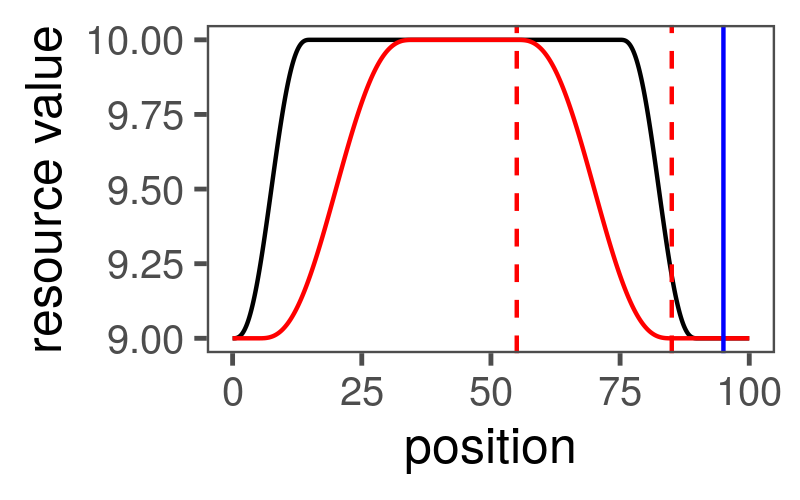
\includegraphics{fig_smootherstep.png}
\caption{Depletion on a wrapped linear landscape by an agent at x = 95
(blue line). Depletion is the departure from the maximum resource value
(10.0). Curves show the \emph{smootherstep} interpolated depletion for
the following parameter combinations: dead zone = 5, depletion range =
20 (black line), and dead zone = 10, depletion range = 40 (red line).
Dashed red vertical lines show the limits of the interpolation for the
second case.}
\end{figure}

There is no resource replenishment within a generation, and
within-generation heterogeneity in resource values arises from agent
foraging. The landscape is replenished by a fixed value each generation,
with a fixed carrying capacity, leading to between-generation
heterogeneity.

\hypertarget{agents}{%
\section{Agents}\label{agents}}

\hypertarget{agent-attributes}{%
\subsection{Agent attributes}\label{agent-attributes}}

The population consists of a fixed number of individuals. Each
individual stores the following information, which is used and updated
during the simulation:

\begin{itemize}
\tightlist
\item
  ANN: An artificial neural network used to assess other individuals.
\item
  Circular position: A value (0.0 -- 1.0) representing a position on the
  wrapped linear landscape. Initially randomly chosen.
\item
  Explore/exploit trade-off: A heritable value (0.0 -- 1.0) representing
  the probability of exploiting a resource value.
\item
  Leader identity: The identity of the agent chosen to follow, if any.
\end{itemize}

\hypertarget{agent-dynamics}{%
\subsection{Agent dynamics}\label{agent-dynamics}}

Each agent makes a single initial movement in each timestep from the
roost to a point on the landscape (circular position). Agents are
created with a position drawn from a uniform distribution.

When making the initial \emph{roost-landscape movement}, the population
is shuffled into a \emph{movement queue}. The first individual in the
queue is assumed to be independent, and has no leader (Figure 2). All
subsequent individuals in the queue must assess whether to follow this
\emph{movement queue leader} to its position on the landscape. This
assessment is described below. The leader and any followers are removed
from the movement queue. The remaining agents are shuffled again to form
another movement queue, and the first agent becomes the new movement
queue leader. The process above repeats until only a single agent
remains in the queue, which is assumed to have no choice but to be
independent.

\begin{figure}
\centering
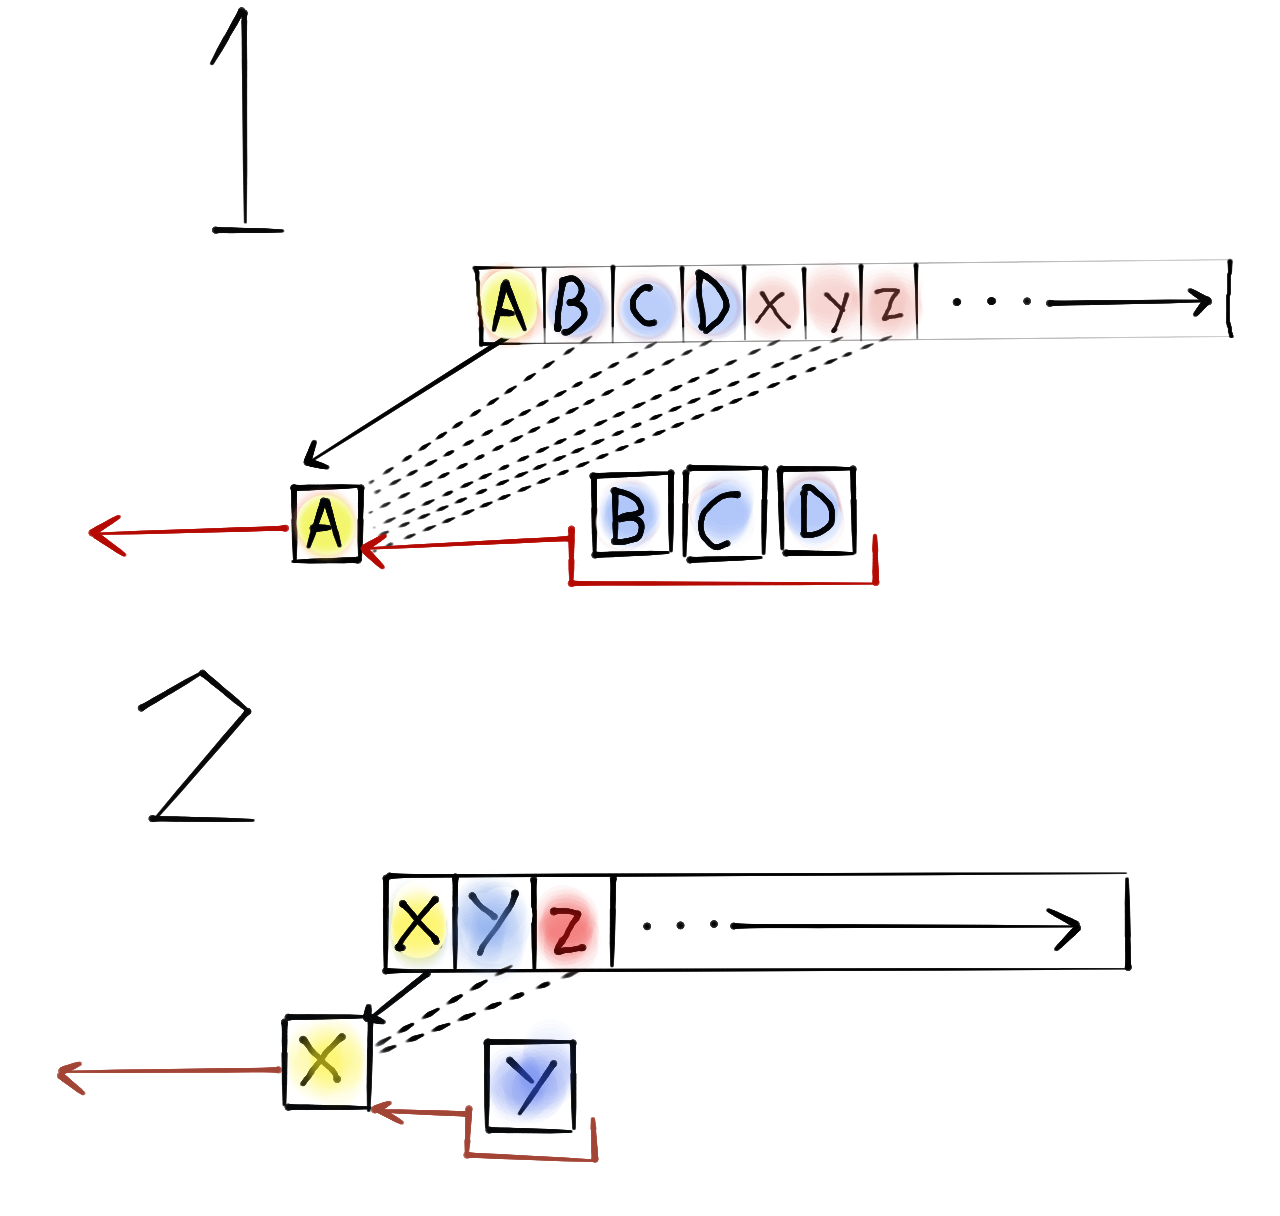
\includegraphics{fig_moveq.png}
\caption{The roost-landscape movement queue dynamic. In step 1, agent A
is the randomly chosen movement queue leader. Agents B -- Z assess A to
follow; and B -- D choose to follow, and A -- D are removed from the
queue. The queue is updated in step 2, with X randomly assigned head of
the reduced queue, and the dynamic repeats.}
\end{figure}

Having made the roost-landscape movement, agents make an
\emph{exploration-exploitation trade-off} over a fixed number of
foraging turns, based on the inherited trade-off parameter (Figure 3).
The trade-off is made until the first (probabilistic) decision to
exploit, or until turns run out. Agents take in resources for as many
turns as remain after choosing to exploit. For turns in which an agent
chooses to explore, it performs a random walk with a step-length 1.0\%
of landscape size, and updates its circular position. Agents that never
exploit are assumed to have no intake. Agents `memorise' their (new)
circular position when they return to the roost at the end of the
timestep.

\begin{figure}
\centering
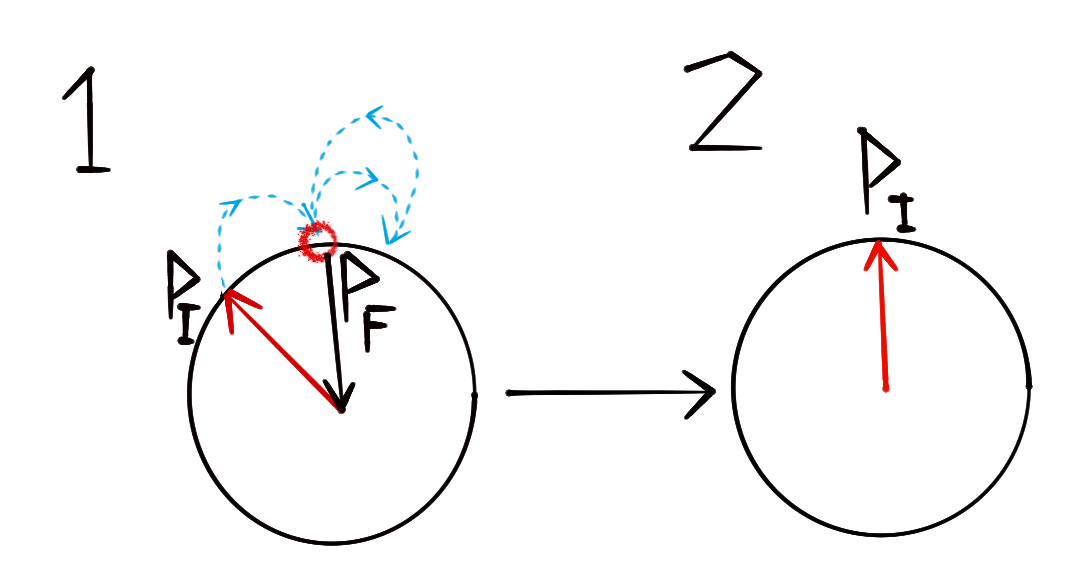
\includegraphics{fig_circmove.png}
\caption{The exploration-exploitation dynamic and agent movement along
the landscape. In step 1, an agent moves to its initial position on the
landscape \(P_I\). From there, it executes a random-walk with a
probability of stopping to exploit specified by the
exploration-exploitation trade-off parameter (dashed blue lines), until
it stops to exploit (red circle, final position \(P_F\)). After
returning to the roost, the agent, if independent, will return to the
previous final position as the new initial position.}
\end{figure}

At the beginning of the next timestep, an independent agent with no
leader moves to the most recently memorised landscape position. In
contrast, follower agents move to the position of their leader, as
described above.

Agents are modelled as asexually reproducing, with a fixed population
size. Total agent intake over a generation is used as a proxy for
fitness, and is always \textgreater{}= 0. A new population is generated
before the old one is destroyed. The neural network node weights and
inherited movement parameter of an agent \emph{j} in the new population
are set to be the same as those of an agent \emph{i} in the old
population, which is considered to be the parent. The probability of any
agent \emph{i} being chosen as the parent is proportional to its share
of the total intake of the population. The neural network weights and
movement parameter values of the new generation undergo random mutation
at a very low rate, 0.001. The value by which each weight, or the
movement value is mutated is drawn from a Cauchy distribution around the
original value.

\begin{figure}
\centering
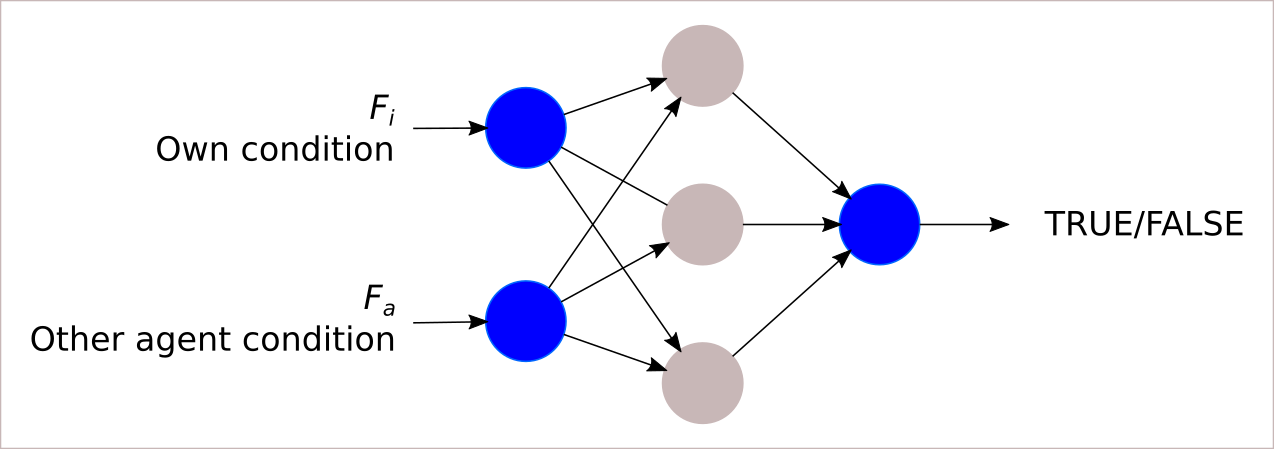
\includegraphics{fig_modesc_infomove.png}
\caption{Artificial neural network (ANN) architecture used in this
model. Agents assess their own condition and that of every other agent
in the population to determine whether or not the assessed individual
should be followed.}
\end{figure}

\hypertarget{leader-assessment}{%
\subsection{Leader assessment}\label{leader-assessment}}

Agent assessment is performed by an artificial neural network with 2
input nodes, a single hidden layer of 3 nodes, and one output node
(Figure 4). All node values are initialised at 0. The two input nodes
are provided the assessing agent's own condition, \(F_i\), and the
assessed agent's condition \(F_a\); \(F_i\) and \(F_a\) are the summed
intakes of the two agents respectively. These may be thought of as body
condition, number of juveniles, return time, or some other indicator of
foraging success. The single output node returns a floating point value
which is assessed as either TRUE (follow) when greater than 0.0, and
FALSE (do not follow) otherwise.

\hypertarget{questions}{%
\section{Questions}\label{questions}}

We aim to answer the following questions:

\begin{enumerate}
\def\labelenumi{\arabic{enumi}.}
\tightlist
\item
  Does the population achieve higher total fitness when information
  transfer is allowed? Do the observed dynamics change when the
  population has \textgreater{} 1 roosting site?
\item
  How does the proportion of followers to leaders change over ecological
  and evolutionary timescales?
\item
  Is the leader-follower dynamic correlated with the explore-exploit
  trade-off?
\end{enumerate}

\hypertarget{model-parameters}{%
\section{Model parameters}\label{model-parameters}}

\begin{longtable}[]{@{}lll@{}}
\toprule
Paramter & Value & Example/Interpretation\tabularnewline
\midrule
\endhead
\textbf{Population} & &\tabularnewline
Generations & 1000 &\tabularnewline
Timesteps & 10 & Tidal cycle, foraging trip\tabularnewline
Population & 100, 1000, 10000 &\tabularnewline
\textbf{Landscape} & &\tabularnewline
Discretisation points & 100 &\tabularnewline
Max resource & 10.0 & Res. carrying capacity\tabularnewline
Res. regrowth & Max/2, variable &\tabularnewline
Foraging turns & 5 & Tidal cycle duration\tabularnewline
Fraction resource depleted & 0.01 &\tabularnewline
\textbf{Artificial neural network} & &\tabularnewline
ANN weights & 0.0 &\tabularnewline
Mutation value & 0.001 &\tabularnewline
Mutation shape & 0.1 Cauchy distribution &\tabularnewline
Architecture & 2 -- 3 -- 1 &\tabularnewline
Node function & Rectified linear activation &\tabularnewline
Network type & Simple feed-forward &\tabularnewline
\bottomrule
\end{longtable}

\hypertarget{references}{%
\section*{References}\label{references}}
\addcontentsline{toc}{section}{References}

\hypertarget{refs}{}
\leavevmode\hypertarget{ref-bijleveld2010}{}%
Bijleveld, Allert I., Martijn Egas, Jan A. Van Gils, and Theunis
Piersma. 2010. ``Beyond the Information Centre Hypothesis: Communal
Roosting for Information on Food, Predators, Travel Companions and
Mates?'' \emph{Oikos} 119 (2): 277--85.
\url{https://doi.org/10.1111/j.1600-0706.2009.17892.x}.

\leavevmode\hypertarget{ref-ebert2003}{}%
Ebert, David S., F. Kenton Musgrave, Darwyn Peachey, Ken Perlin, and
Steven Worley. 2003. \emph{Texturing \& Modeling: A Procedural
Approach}. Morgan Kaufmann.

\leavevmode\hypertarget{ref-harelroi2017}{}%
Harel Roi, Spiegel Orr, Getz Wayne M., and Nathan Ran. 2017. ``Social
Foraging and Individual Consistency in Following Behaviour: Testing the
Information Centre Hypothesis in Free-Ranging Vultures.''
\emph{Proceedings of the Royal Society B: Biological Sciences} 284
(1852): 20162654. \url{https://doi.org/10.1098/rspb.2016.2654}.

\leavevmode\hypertarget{ref-ward1973}{}%
Ward, P., and A. Zahavi. 1973. ``The Importance of Certain Assemblages
of Birds as `Information-Centres' for Food-Finding.'' \emph{Ibis} 115
(4): 517--34. \url{https://doi.org/10.1111/j.1474-919X.1973.tb01990.x}.
